\documentclass{beamer}
\usepackage[MeX]{polski} 
\title{Prezentacja Ptaki}
\author{Aleksy Stocki}
\institute{Uniwersytet Gdański}
\date{2023}
\usetheme{Antibes}
\usecolortheme{crane}
\usepackage{adjustbox}
\graphicspath{ {./zdjecia/} }
\renewcommand{\footnotesize}{\tiny} 

\begin{document}
	
	\frame{\titlepage}
	\begin{frame}
		\frametitle{Table of Contents}
		\tableofcontents
	\end{frame}

\section{Bociany}
	\begin{frame}
		\frametitle{Bociany}
		Bocian biały (Ciconia ciconia) – gatunek dużego ptaka brodzącego z rodziny bocianów (Ciconiidae).
Jego upierzenie jest głównie białe, z czarnymi piórami na skrzydłach. Dorosłe ptaki mają długie, czerwone nogi oraz długie, spiczasto zakończone, czerwone dzioby. Mierzą średnio 100–115 cm od czubka dzioba do końca ogona, ze skrzydłami o rozpiętości 155–215 cm. Bociany mają różne dzioby
		\begin{enumerate}
			\item Bocian Biały
			\item Bocian Czarnodzioby
			\item Bocian Sinodzioby
		\end{enumerate}
		Bocian biały podejmuje co roku dalekie wędrówki, zimując w Afryce, od tropikalnej Afryki Subsaharyjskiej po Republikę Południowej Afryki na południu lub na subkontynencie indyjskim (podgatunek azjatycki).
	\end{frame}

\section{Bociany \& Pożywienie}
	\begin{frame}{Pożywienie}
		Będąc mięsożercą, bocian biały zjada szereg zwierząt, w tym owady, ryby, płazy, gady, małe ssaki i małe ptaki. Większość ze swojego pożywienia znajduje na podłożu, wśród niskiej roślinności oraz w płytkich wodach.\footnotemark
		Dieta bocianów białych jest zróżnicowana w zależności od pory roku, regionu i dostępności pożywienia. Do typowego pożywienia zalicza się owady, dżdżownice, gady, płazy oraz male ssaki
		\begin{table}
			\hfill
		\begin{tabular}{|c||c||c|}
			\hline
			Bociany & Plazy& Stawonogi \\ 
			\hline
			Bocian Biały & żaba wodna & szarańcze\\ 
			\hline
			Bocian Czarnodzioby & żaba trawna & świerszczet\\ 
			\hline
		\end{tabular}
		\end{table}
	\footnotetext[1]{Wiki Pedia,``Wikipedia" \emph{Genialne artykuły za darmo}}
	\end{frame}

\section{Kruk}
	\begin{frame}
		\frametitle{Kruk zwyczajny}
			 gatunek dużego osiadłego ptaka z rodziny krukowatych (Corvidae). Występuje na półkuli północnej, jest najbardziej rozpowszechnionym gatunkiem spośród wszystkich krukowatych. Obecnie wyróżnia się jedenaście podgatunków
\footnotemark
		\begin{columns}[t]
			\begin{column}{.5\textwidth}
				\adjincludegraphics[width=.8\linewidth, valign=t]{kruk.jpg}
				\label{fig: kruk}
			\end{column}
			\begin{column}{.5\textwidth}
				\\\begin{itemize}
					\item Kruk pustynny
					\item Kruk srokaty
					\item Kruk meksykański
					\item Kruk tasmański
				\end{itemize}
			\end{column}
		\end{columns}
	\footnotetext[2]{Goog Le, ``Google" \emph{Cudowne zdjęcia}}
	\end{frame}

\section{Co wcina kruk?}
	\begin{frame}
		\frametitle{Różne rzeczy}
		Wszystkożerny, jednak głównie pokarm zwierzęcy – drobne ssaki, żaby i inne płazy, jaszczurki i inne gady, ptaki, w tym ich młode i jaja, owady, dżdżownice, robaki, ślimaki, padlina, szczególnie zimą i w górach, również odpadki ze śmietników. Czasem zjada też różne nasiona, żołędzie, pąki roślin i owoce, choć tylko w ramach uzupełnienia diety.
Żeruje głównie na ziemi. 
		\begin{figure}[H]
			\centering
			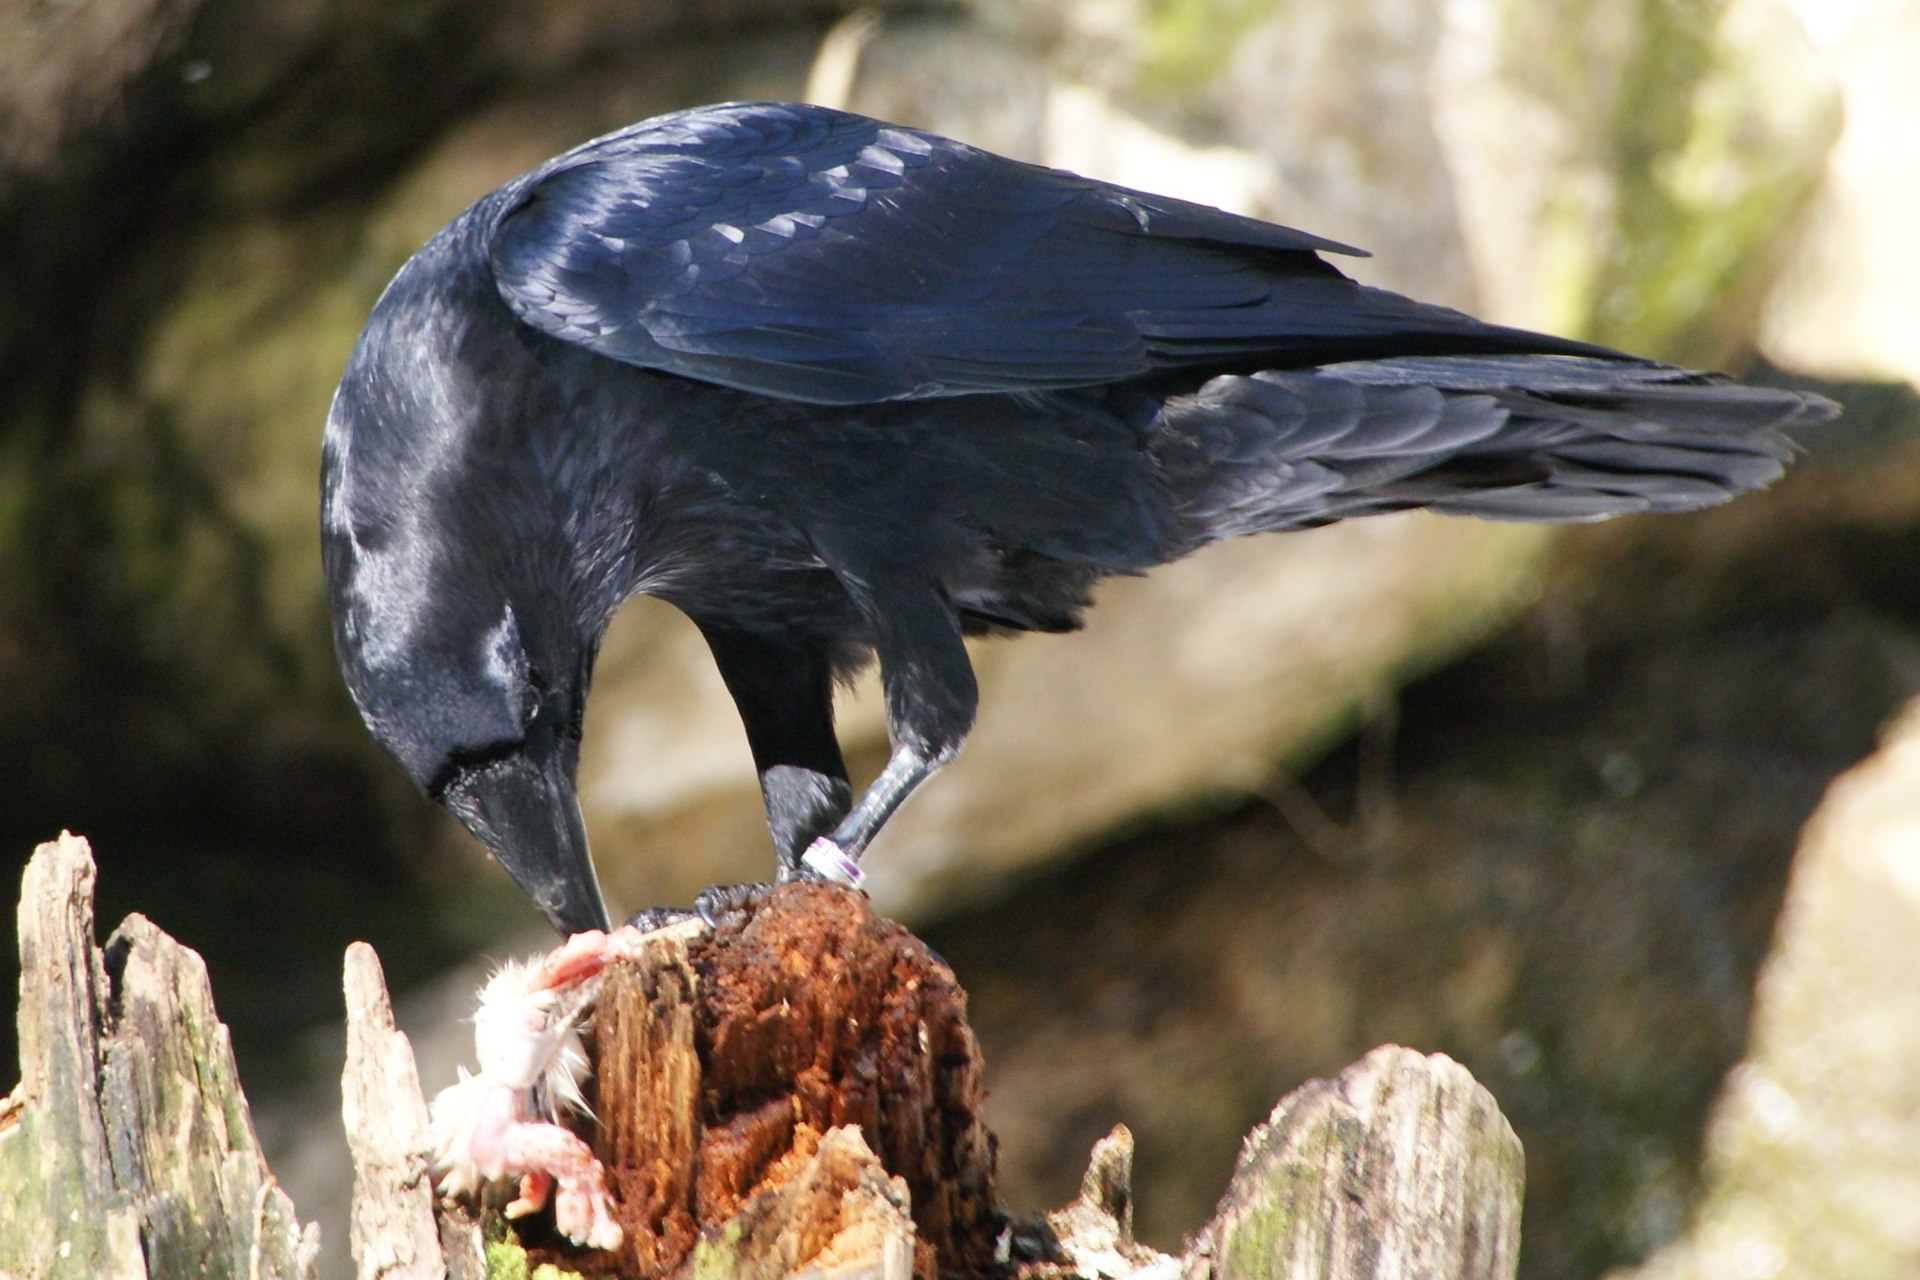
\includegraphics[width=5cm, height=1.5cm]{kruk_je.jpg}
			\caption{Kruk jedzący}
			\label{fig: wcina}
		\end{figure}
		Jednym z pokarmowych niebezpieczeństw czyhającym na ptaka ze strony człowieka są zatrute jaja wykładane po to, by zlikwidować szkodniki.
	\end{frame}

\section{Dzięcioł duży}
	\begin{frame}
		\frametitle{Dzięciołek}
			\begin{columns}[t]
				\begin{column}{.5\textwidth}
					\\\adjincludegraphics[width=.8\linewidth, valign=t]{dzieciol.jpg}
					\newline
					\label{fig: dzieciol}
				\end{column}
				\begin{column}{.5\textwidth}
					\begin{enumerate}
						\item Jest wielkości drozda
						\item ściśle związany z korowiną drzew
						\item czerwone tęczówki oczu
						\item nie jest płochliwy
						\item jego lot jest falisty
					\end{enumerate}
				\end{column}
			\end{columns}
			W okresie wiosny i lata, jego pożywienie stanowią głównie owady i ich larwy wydobywane z drewna~\ref{fig: wcina}
	\end{frame}


\begin{frame}{Lista różnych ptaków}
\begin{columns}[T]
	\column{0.99\textwidth}
	\begin{itemize}
		\item Wróbel
		\item Sikorka
		\item Czapla
		\item Tukan
		\item Pelikan
		\item Trzewikodziób
	\end{itemize}
	
	\column{0.01\textwidth}
	\hspace*{-5cm}
	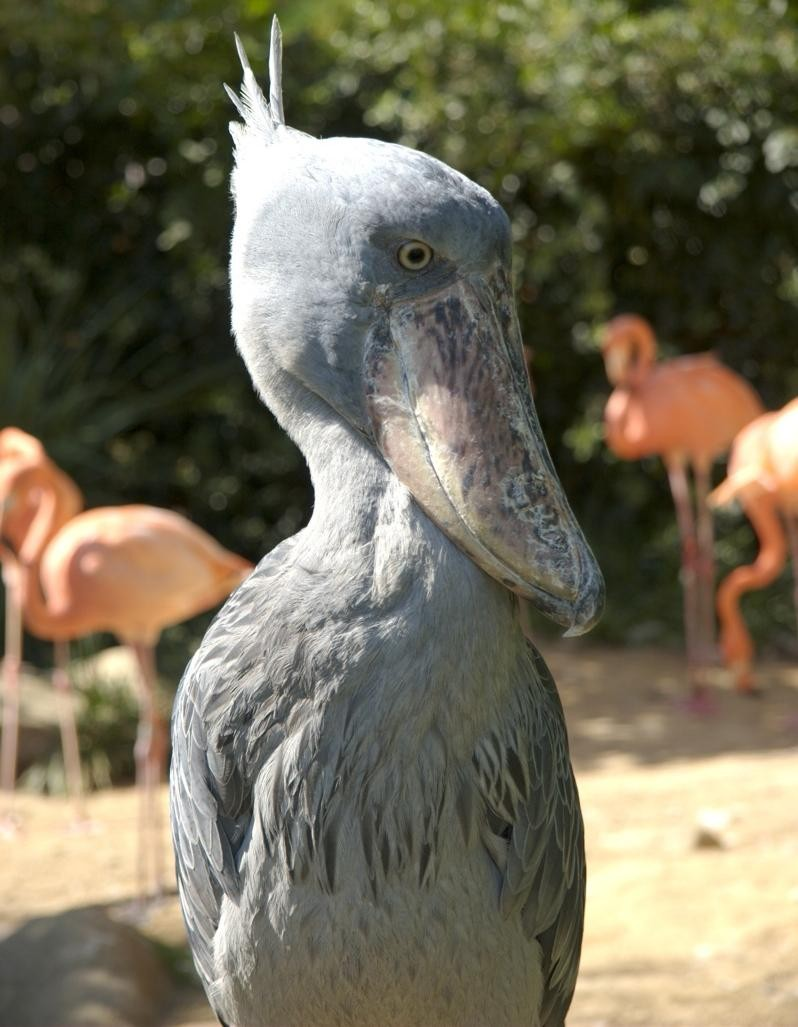
\includegraphics[width=5cm]{shoebill.jpg}
\end{columns}
\end{frame}


\begin{frame}{Trzewikodziób}
 gatunek dużego ptaka z rodziny trzewikodziobów (Balaenicipitidae), będący jej jedynym przedstawicielem. Występuje od Sudanu Południowego i południowo-zachodniej Etiopii przez Ugandę po południowo-wschodnią Demokratyczną Republikę Konga i północną Zambię.
	\begin{columns}
		\column{0.1\textwidth}
		\begin{figure}
			\hspace*{-3cm}
			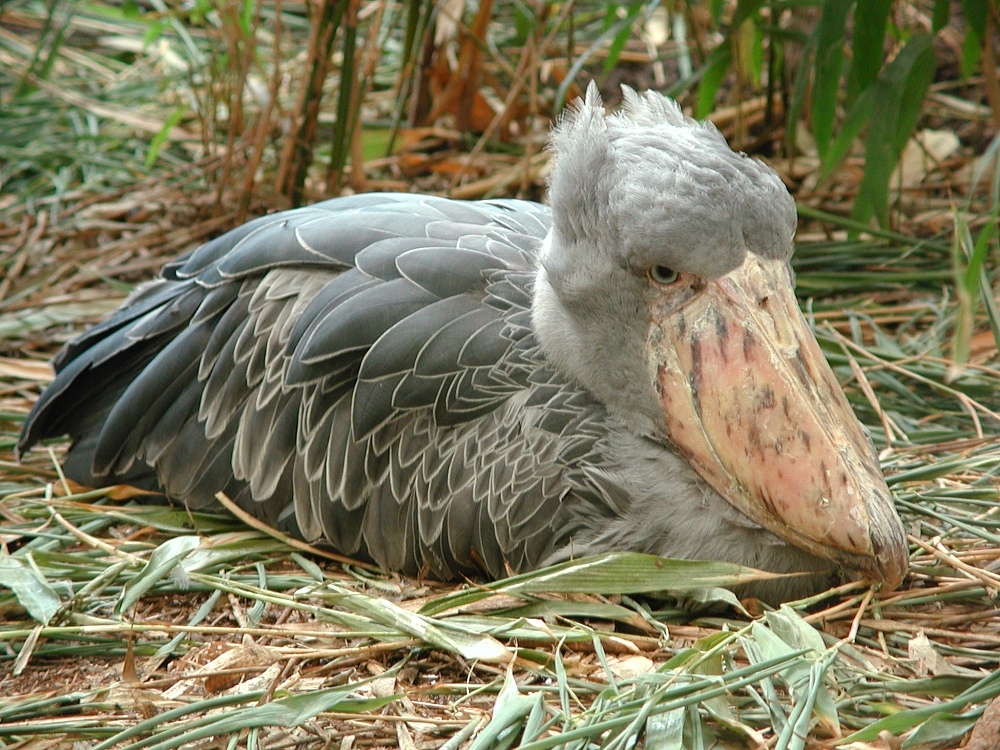
\includegraphics[width=4cm]{czilera.jpg}
			\caption{czil}
		\end{figure}
		
		\column{0.01\textwidth}
		\begin{figure}
			\caption{c:}
			\hspace*{-2cm}
			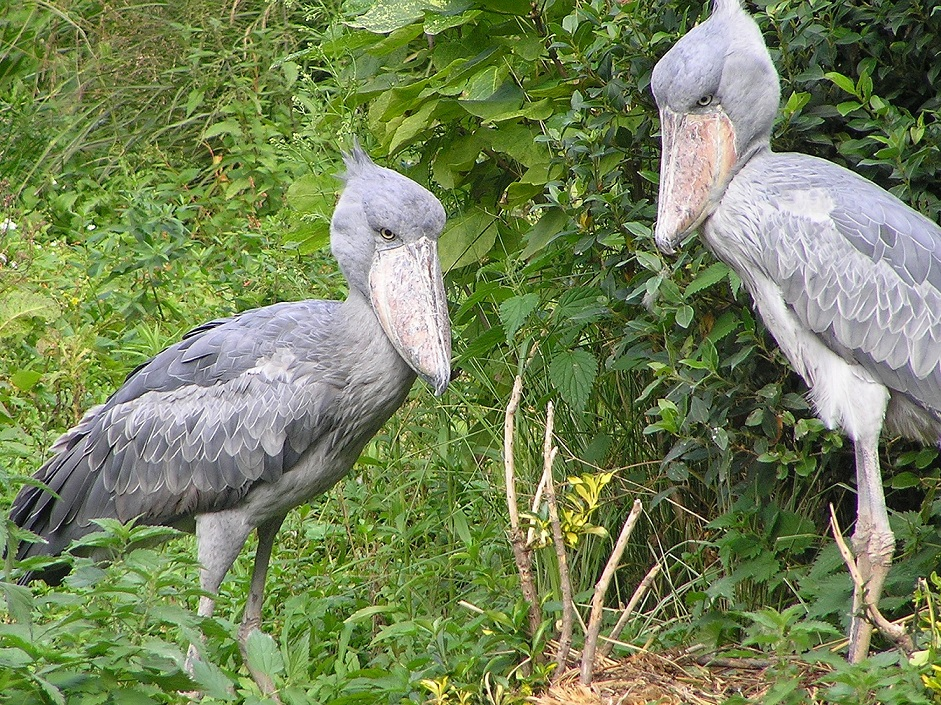
\includegraphics[width=4cm]{kolezanka.jpg}
			
		\end{figure}
	\end{columns}
\end{frame}

\section{Sources}
\begin{frame}{Bibliografia}
\begin{thebibliography}{10}
	\bibitem{Wiki}Wiki Pedia, ``Wikipedia" \emph{Genialne artykuły za darmo}, pp. 201, Jan 2023.
	\bibitem{Google}Goog Le, ``Google," \emph{Cudowne zdjęcia}, pp. 105, Jan 2023.
\end{thebibliography}
\end{frame}



\end{document}